\documentclass[margin=5mm]{standalone}
\usepackage[dvipsnames]{xcolor}
\usepackage{pgfplots}
\usepackage{tikz}
\usepackage[tikz]{ocgx2}

\pgfplotsset{compat=1.18}
\begin{document}

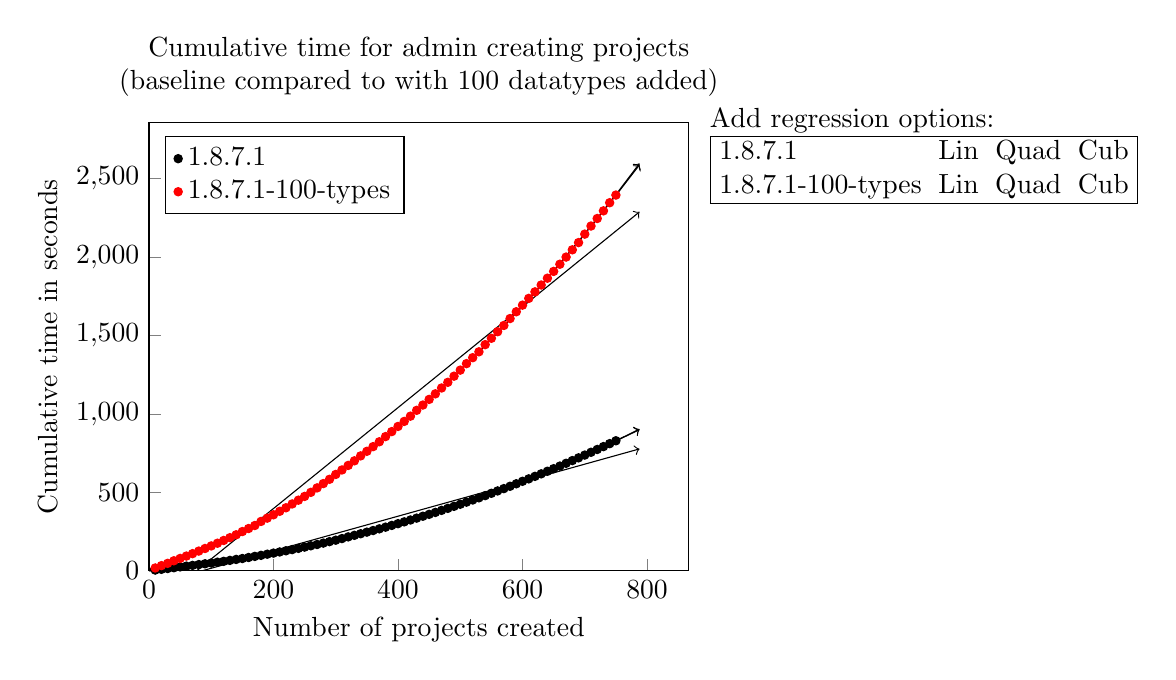
\begin{tikzpicture}
    \begin{axis}[
        align = center,
        legend pos = north west,
        legend cell align = left,
        xlabel = Number of projects created,
        ylabel = Cumulative time in seconds,
        xtick pos = left,
        ytick pos = left,
        scaled ticks = false,
        xmin = 0,
        ymin = 0,
        title = {Cumulative time for admin creating projects (baseline compared to with 100 datatypes added)},
        title style = {text width = 0.8\textwidth},
        legend entries={\switchocg{1.8.7.1}{1.8.7.1},\switchocg{1.8.7.1-100-types}{1.8.7.1-100-types}}]
        \begin{scope}[ocg = {ref = 1.8.7.1-Lin, status = invisible}]
            \plot[domain=0:788,->,forget plot] (\x,{-93.4087935135136575581782381050288677215576171875 + 1.1047842987197726838388689429848454892635345458984375*(\x)^1});
        \end{scope}
        \begin{scope}[ocg = {ref = 1.8.7.1-Quad, status = invisible}]
            \plot[domain=0:788,->,forget plot] (\x,{6.67915591262458807619850631454028189182281494140625 + 0.3248781992953182484740182189852930605411529541015625*(\x)^1 + 0.0010261922360848088099649633164744955138303339481353759765625*(\x)^2});
        \end{scope}
        \begin{scope}[ocg = {ref = 1.8.7.1-Cub, status = invisible}]
            \plot[domain=0:788,->,forget plot] (\x,{4.4908741725281995371688026352785527706146240234375 + 0.358327380283190721765862463144003413617610931396484375*(\x)^1 + 0.0009168874538622137811139101160051723127253353595733642578125*(\x)^2 + 0.0000000958813879145569689221710076021398805323769920505583286285400390625*(\x)^3});
        \end{scope}
        \begin{scope}[ocg = {ref = 1.8.7.1, status = visible}]
            \addplot[
                only marks,
                color = black,
                mark = *,
                mark size = 1.5 pt
            ]coordinates {(10,5.616)(20,10.359)(30,15.385)(40,20.348)(50,25.887)(60,30.672)(70,35.361)(80,40.462)(90,45.493)(100,50.451)(110,55.648)(120,61.19)(130,67.113)(140,73.251)(150,79.087)(160,85.612)(170,92.619)(180,99.247)(190,106.661)(200,113.677)(210,120.809)(220,128.363)(230,135.843)(240,143.716)(250,151.76)(260,160.183)(270,168.371)(280,177.304)(290,186.64)(300,195.784)(310,206.171)(320,216.814)(330,226.848)(340,236.869)(350,247.029)(360,257.284)(370,268.132)(380,278.756)(390,289.953)(400,301.108)(410,312.545)(420,324.376)(430,336.295)(440,348.352)(450,360.353)(460,372.582)(470,385.73)(480,398.458)(490,411.36)(500,424.59)(510,438.084)(520,451.737)(530,465.54)(540,479.561)(550,494.461)(560,509.408)(570,524.241)(580,539.186)(590,555.041)(600,570.8)(610,586.325)(620,602.159)(630,618.315)(640,634.705)(650,651.027)(660,667.642)(670,685.466)(680,702.653)(690,720.11)(700,737.7)(710,755.563)(720,773.397)(730,791.724)(740,810.486)(750,828.845)};
        \end{scope}
        \begin{scope}[ocg = {ref = 1.8.7.1-100-types-Lin, status = invisible}]
            \plot[domain=0:788,->,forget plot] (\x,{-245.15396936936946303831064142286777496337890625 + 3.212710480796586498541955734253861010074615478515625*(\x)^1});
        \end{scope}
        \begin{scope}[ocg = {ref = 1.8.7.1-100-types-Quad, status = invisible}]
            \plot[domain=0:788,->,forget plot] (\x,{6.56886938170981427020933551830239593982696533203125 + 1.251233815203759203171784974983893334865570068359375*(\x)^1 + 0.002580890349464247217337042883400499704293906688690185546875*(\x)^2});
        \end{scope}
        \begin{scope}[ocg = {ref = 1.8.7.1-100-types-Cub, status = invisible}]
            \plot[domain=0:788,->,forget plot] (\x,{12.6398381471874490244999833521433174610137939453125 + 1.1584354660299265304956861655227839946746826171875*(\x)^1 + 0.0028841355425450513304264088532136156572960317134857177734375*(\x)^2 + -0.0000002660045553340387510467724037355186084141678293235599994659423828125*(\x)^3});
        \end{scope}
        \begin{scope}[ocg = {ref = 1.8.7.1-100-types, status = visible}]
            \addplot[
                only marks,
                color = red,
                mark = *,
                mark size = 1.5 pt
            ]coordinates {(10,18.873)(20,33.798)(30,48.391)(40,64.747)(50,79.592)(60,94.712)(70,110.058)(80,126.405)(90,142.933)(100,159.304)(110,176.48)(120,194.147)(130,211.863)(140,230.126)(150,250.833)(160,270.014)(170,289.319)(180,315.21)(190,336.266)(200,357.539)(210,379.862)(220,402.166)(230,426.67)(240,450.563)(250,474.57)(260,500.45)(270,528.766)(280,556.236)(290,583.518)(300,614.426)(310,642.985)(320,671.928)(330,701.192)(340,732.556)(350,761.704)(360,791.567)(370,822.453)(380,855.412)(390,887.335)(400,919.994)(410,952.088)(420,985.599)(430,1022.765)(440,1056.404)(450,1092.147)(460,1127.731)(470,1164.921)(480,1201.029)(490,1240.171)(500,1278.689)(510,1320.025)(520,1357.896)(530,1395.346)(540,1440.891)(550,1481.579)(560,1523.294)(570,1563.038)(580,1607.105)(590,1650.321)(600,1692.409)(610,1735.447)(620,1776.975)(630,1820.66)(640,1863.936)(650,1907.288)(660,1952.992)(670,1998.501)(680,2044.772)(690,2090.719)(700,2144.685)(710,2196.295)(720,2244.162)(730,2292.861)(740,2344.642)(750,2393.355)};
        \end{scope}
    \end{axis}
    \begin{scope}
        \addtolength{\tabcolsep}{-0.3em}
        \node [below right, shape=rectangle, align=left](regressiontable) at (7,6) {
            Add regression options: \\
            \begin{tabular}{|llll|}
                \hline
                1.8.7.1 & \switchocg{1.8.7.1-Lin}{Lin} & \switchocg{1.8.7.1-Quad}{Quad} & \switchocg{1.8.7.1-Cub}{Cub} \\
                1.8.7.1-100-types & \switchocg{1.8.7.1-100-types-Lin}{Lin} & \switchocg{1.8.7.1-100-types-Quad}{Quad} & \switchocg{1.8.7.1-100-types-Cub}{Cub} \\
                \hline
            \end{tabular}
        };
    \end{scope}
\end{tikzpicture}

\end{document}